
%% report.tex
%% 2015 Dec
%% by Matt Vernacchia
%% based on template
%% by Michael Shell
%% See:
%% http://www.michaelshell.org/
%% for current contact information.
%%
%% This is a skeleton file demonstrating the use of IEEEtran.cls
%% (requires IEEEtran.cls version 1.8b or later) with an IEEE
%% conference paper.
%%
%% Support sites:
%% http://www.michaelshell.org/tex/ieeetran/
%% http://www.ctan.org/pkg/ieeetran
%% and
%% http://www.ieee.org/


\documentclass[conference]{IEEEtran}

% Some very useful LaTeX packages include:
% (uncomment the ones you want to load)


% *** MISC UTILITY PACKAGES ***
%
%\usepackage{ifpdf}
% Heiko Oberdiek's ifpdf.sty is very useful if you need conditional
% compilation based on whether the output is pdf or dvi.
% usage:
% \ifpdf
%   % pdf code
% \else
%   % dvi code
% \fi
% The latest version of ifpdf.sty can be obtained from:
% http://www.ctan.org/pkg/ifpdf
% Also, note that IEEEtran.cls V1.7 and later provides a builtin
% \ifCLASSINFOpdf conditional that works the same way.
% When switching from latex to pdflatex and vice-versa, the compiler may
% have to be run twice to clear warning/error messages.






% *** CITATION PACKAGES ***
%
%\usepackage{cite}
% cite.sty was written by Donald Arseneau
% V1.6 and later of IEEEtran pre-defines the format of the cite.sty package
% \cite{} output to follow that of the IEEE. Loading the cite package will
% result in citation numbers being automatically sorted and properly
% "compressed/ranged". e.g., [1], [9], [2], [7], [5], [6] without using
% cite.sty will become [1], [2], [5]--[7], [9] using cite.sty. cite.sty's
% \cite will automatically add leading space, if needed. Use cite.sty's
% noadjust option (cite.sty V3.8 and later) if you want to turn this off
% such as if a citation ever needs to be enclosed in parenthesis.
% cite.sty is already installed on most LaTeX systems. Be sure and use
% version 5.0 (2009-03-20) and later if using hyperref.sty.
% The latest version can be obtained at:
% http://www.ctan.org/pkg/cite
% The documentation is contained in the cite.sty file itself.






% *** GRAPHICS RELATED PACKAGES ***
%
\ifCLASSINFOpdf
  \usepackage[pdftex]{graphicx}
  % declare the path(s) where your graphic files are
  % \graphicspath{{../pdf/}{../jpeg/}}
  % and their extensions so you won't have to specify these with
  % every instance of \includegraphics
  % \DeclareGraphicsExtensions{.pdf,.jpeg,.png}
\else
  % or other class option (dvipsone, dvipdf, if not using dvips). graphicx
  % will default to the driver specified in the system graphics.cfg if no
  % driver is specified.
  % \usepackage[dvips]{graphicx}
  % declare the path(s) where your graphic files are
  % \graphicspath{{../eps/}}
  % and their extensions so you won't have to specify these with
  % every instance of \includegraphics
  % \DeclareGraphicsExtensions{.eps}
\fi
% graphicx was written by David Carlisle and Sebastian Rahtz. It is
% required if you want graphics, photos, etc. graphicx.sty is already
% installed on most LaTeX systems. The latest version and documentation
% can be obtained at: 
% http://www.ctan.org/pkg/graphicx
% Another good source of documentation is "Using Imported Graphics in
% LaTeX2e" by Keith Reckdahl which can be found at:
% http://www.ctan.org/pkg/epslatex
%
% latex, and pdflatex in dvi mode, support graphics in encapsulated
% postscript (.eps) format. pdflatex in pdf mode supports graphics
% in .pdf, .jpeg, .png and .mps (metapost) formats. Users should ensure
% that all non-photo figures use a vector format (.eps, .pdf, .mps) and
% not a bitmapped formats (.jpeg, .png). The IEEE frowns on bitmapped formats
% which can result in "jaggedy"/blurry rendering of lines and letters as
% well as large increases in file sizes.
%
% You can find documentation about the pdfTeX application at:
% http://www.tug.org/applications/pdftex





% *** MATH PACKAGES ***
%
\usepackage{amsmath}
% A popular package from the American Mathematical Society that provides
% many useful and powerful commands for dealing with mathematics.
%
% Note that the amsmath package sets \interdisplaylinepenalty to 10000
% thus preventing page breaks from occurring within multiline equations. Use:
%\interdisplaylinepenalty=2500
% after loading amsmath to restore such page breaks as IEEEtran.cls normally
% does. amsmath.sty is already installed on most LaTeX systems. The latest
% version and documentation can be obtained at:
% http://www.ctan.org/pkg/amsmath





% *** SPECIALIZED LIST PACKAGES ***
%
\usepackage{algorithmicx}
% algorithmic.sty was written by Peter Williams and Rogerio Brito.
% This package provides an algorithmic environment fo describing algorithms.
% You can use the algorithmic environment in-text or within a figure
% environment to provide for a floating algorithm. Do NOT use the algorithm
% floating environment provided by algorithm.sty (by the same authors) or
% algorithm2e.sty (by Christophe Fiorio) as the IEEE does not use dedicated
% algorithm float types and packages that provide these will not provide
% correct IEEE style captions. The latest version and documentation of
% algorithmic.sty can be obtained at:
% http://www.ctan.org/pkg/algorithms
% Also of interest may be the (relatively newer and more customizable)
% algorithmicx.sty package by Szasz Janos:
% http://www.ctan.org/pkg/algorithmicx




% *** ALIGNMENT PACKAGES ***
%
\usepackage{array}
% Frank Mittelbach's and David Carlisle's array.sty patches and improves
% the standard LaTeX2e array and tabular environments to provide better
% appearance and additional user controls. As the default LaTeX2e table
% generation code is lacking to the point of almost being broken with
% respect to the quality of the end results, all users are strongly
% advised to use an enhanced (at the very least that provided by array.sty)
% set of table tools. array.sty is already installed on most systems. The
% latest version and documentation can be obtained at:
% http://www.ctan.org/pkg/array


% IEEEtran contains the IEEEeqnarray family of commands that can be used to
% generate multiline equations as well as matrices, tables, etc., of high
% quality.




% *** SUBFIGURE PACKAGES ***
%\ifCLASSOPTIONcompsoc
%  \usepackage[caption=false,font=normalsize,labelfont=sf,textfont=sf]{subfig}
%\else
%  \usepackage[caption=false,font=footnotesize]{subfig}
%\fi
% subfig.sty, written by Steven Douglas Cochran, is the modern replacement
% for subfigure.sty, the latter of which is no longer maintained and is
% incompatible with some LaTeX packages including fixltx2e. However,
% subfig.sty requires and automatically loads Axel Sommerfeldt's caption.sty
% which will override IEEEtran.cls' handling of captions and this will result
% in non-IEEE style figure/table captions. To prevent this problem, be sure
% and invoke subfig.sty's "caption=false" package option (available since
% subfig.sty version 1.3, 2005/06/28) as this is will preserve IEEEtran.cls
% handling of captions.
% Note that the Computer Society format requires a larger sans serif font
% than the serif footnote size font used in traditional IEEE formatting
% and thus the need to invoke different subfig.sty package options depending
% on whether compsoc mode has been enabled.
%
% The latest version and documentation of subfig.sty can be obtained at:
% http://www.ctan.org/pkg/subfig




% *** FLOAT PACKAGES ***
%
%\usepackage{fixltx2e}
% fixltx2e, the successor to the earlier fix2col.sty, was written by
% Frank Mittelbach and David Carlisle. This package corrects a few problems
% in the LaTeX2e kernel, the most notable of which is that in current
% LaTeX2e releases, the ordering of single and double column floats is not
% guaranteed to be preserved. Thus, an unpatched LaTeX2e can allow a
% single column figure to be placed prior to an earlier double column
% figure.
% Be aware that LaTeX2e kernels dated 2015 and later have fixltx2e.sty's
% corrections already built into the system in which case a warning will
% be issued if an attempt is made to load fixltx2e.sty as it is no longer
% needed.
% The latest version and documentation can be found at:
% http://www.ctan.org/pkg/fixltx2e


%\usepackage{stfloats}
% stfloats.sty was written by Sigitas Tolusis. This package gives LaTeX2e
% the ability to do double column floats at the bottom of the page as well
% as the top. (e.g., "\begin{figure*}[!b]" is not normally possible in
% LaTeX2e). It also provides a command:
%\fnbelowfloat
% to enable the placement of footnotes below bottom floats (the standard
% LaTeX2e kernel puts them above bottom floats). This is an invasive package
% which rewrites many portions of the LaTeX2e float routines. It may not work
% with other packages that modify the LaTeX2e float routines. The latest
% version and documentation can be obtained at:
% http://www.ctan.org/pkg/stfloats
% Do not use the stfloats baselinefloat ability as the IEEE does not allow
% \baselineskip to stretch. Authors submitting work to the IEEE should note
% that the IEEE rarely uses double column equations and that authors should try
% to avoid such use. Do not be tempted to use the cuted.sty or midfloat.sty
% packages (also by Sigitas Tolusis) as the IEEE does not format its papers in
% such ways.
% Do not attempt to use stfloats with fixltx2e as they are incompatible.
% Instead, use Morten Hogholm'a dblfloatfix which combines the features
% of both fixltx2e and stfloats:
%
% \usepackage{dblfloatfix}
% The latest version can be found at:
% http://www.ctan.org/pkg/dblfloatfix




% *** PDF, URL AND HYPERLINK PACKAGES ***
%
%\usepackage{url}
% url.sty was written by Donald Arseneau. It provides better support for
% handling and breaking URLs. url.sty is already installed on most LaTeX
% systems. The latest version and documentation can be obtained at:
% http://www.ctan.org/pkg/url
% Basically, \url{my_url_here}.

% *** Other packages ***
\usepackage{siunitx}
\usepackage{algpseudocode}
\usepackage{algorithm}
\usepackage{physics}
\usepackage{amsfonts}

% Custom commands for statistics
\newcommand{\E}{\mathrm{E}}
\newcommand{\Var}{\mathrm{Var}}
\newcommand{\Cov}{\mathrm{Cov}}


% *** Do not adjust lengths that control margins, column widths, etc. ***
% *** Do not use packages that alter fonts (such as pslatex).         ***
% There should be no need to do such things with IEEEtran.cls V1.6 and later.
% (Unless specifically asked to do so by the journal or conference you plan
% to submit to, of course. )


% correct bad hyphenation here
\hyphenation{op-tical net-works semi-conduc-tor}


\begin{document}
%
% paper title
% Titles are generally capitalized except for words such as a, an, and, as,
% at, but, by, for, in, nor, of, on, or, the, to and up, which are usually
% not capitalized unless they are the first or last word of the title.
% Linebreaks \\ can be used within to get better formatting as desired.
% Do not put math or special symbols in the title.
\title{Unscented Kalman Filter for 3D Attitude Estimation\\16.322 Final Project}


% author names and affiliations
% use a multiple column layout for up to three different
% affiliations
\author{\IEEEauthorblockN{Matthew Vernacchia}
\IEEEauthorblockA{Department of Aeronautics and Astronautics\\
Massachusetts Institute of Technology\\
Email: mvernacc@mit.edu}}


% make the title area
\maketitle

% As a general rule, do not put math, special symbols or citations
% in the abstract
\begin{abstract}
The abstract goes here.
\end{abstract}

% no keywords




% For peer review papers, you can put extra information on the cover
% page as needed:
% \ifCLASSOPTIONpeerreview
% \begin{center} \bfseries EDICS Category: 3-BBND \end{center}
% \fi
%
% For peerreview papers, this IEEEtran command inserts a page break and
% creates the second title. It will be ignored for other modes.
\IEEEpeerreviewmaketitle



\section{Introduction}
The estimation of an object's 3D pose (rotation and translation) relative to a global reference frame is an important problem in robotics and aerospace engineering. This estimation task is called navigation. Satellites, launch vehicles, manned aircraft and UAVs need pose information in order to control their trajectories and to point sensors, communications equipment and weapons at targets. In this project, I restrict the navigation task to estimating rotation only.\\

Two broad classes of sensors are used in navigation: proprioceptive and exteroceptive \cite{Trawny05quat,Kelly-2010-711}. Proprioceptive sensors measure quantities internal to the robot or vehicle; exteroceptive senors measure the surrounding world.\\

Accelerometers and rate gyroscopes are common proprioceptive sensors; they measure the acceleration and angular velocity of the vehicle body. The sensors detect the effect of non-inertial fictitious forces on the motion of a small system (oscillating mass, spinning wheel, etc.) within the sensor. Typically, three orthogonal gyroscopes and three orthogonal accelerometers are combined into a single device, called a strapdown Inertial Measurement Unit (IMU) \cite{UCAM-CL-TR-696}.\\

In articulated robots or vehicles, proprioceptive sensors are also used to sense joint angles and actuator positions.\\

Navigation can be performed by integrating IMU measurements. However, noise and sensor biases cause the integrated estimate to drift over time. Depending on the quality of the sensors, the estimate becomes useless after tens of seconds (MEMS devices) to several hours (navigation-grade IMUs) \cite{UCAM-CL-TR-696}.\\

To correct for drift, exteroceptive measurements are incorporated into the estimate. Exteroceptive navigation sensors include:
\begin{itemize}
  \item \emph{Field sensors} measure orientation relative to a vector field which has a known direction in the global frame. Magnetometers measure the Earth's magnetic field, and accelerometers can measure the gravitational field (on a non-free-falling vehicle). Note that these sensors cannot detect rotation about the vector, e.g. a gravitational sensor cannot provide yaw/heading information.

  \item \emph{Beacon/Landmark sensors} measure the range and/or bearing to a set of beacons. Examples include Sun sensors \cite{sun-sense}, GPS/GNSS, and LORAN.

  \item \emph{Mapping sensors} sense nearby visual or shape features and match them to a map of the environment. Cameras, LiDAR, and ultrasound rangefinders have been used for mapping. The map can be known a priori, or the estimator can perform simultaneous localization and mapping (SLAM) \cite{AHuangISRR11}.

  \item \emph{Odometry sensors} measure the incremental motion of the vehicle relative to the environment. On wheeled vehicles, encoders are used to count wheel revolutions. \emph{Visual odometry} uses optical flow algorithms to compute motion from camera data \cite{Dille_2009_6430}.
\end{itemize}

In this project, I use an IMU and magnetometer.\\

Several estimators are used in navigation, generally depending on which sensors are available. Non-linear Kalman filters are the typical choice for systems with field, beacon and odometry sensors. Kalman filters work well for systems with approximately Gaussian sensor noise, which these sensors usually have. Mapping sensors require more sophisticated estimators because their measurement distributions are non-Gaussian (e.g. an environment with several similar-looking regions will produce a multi-modal distribution), particle filters are often used in this case.\\

 In this project, I will use an Unscented Kalman filter (UKF). I choose the UKF over the Extended Kalman filter because it offers superior covariance estimation, and avoid the need to determine the Jacobians of the state transition and measurement functions.\\ 

\section{Hardware}
For my sensors, I use an MPU-9150 from InvenSense \cite{mpu9150}. SparkFun Electronics sells the sensor conveniently mounted on a breakout board (part number SEN-11486). The MPU-9150 contains a 3-axis MEMS rate gyro, 3-axis MEMS accelerometer, and a 3-axis Hall effect magnetometer.\\
For computation I use a BeagleBone Black single board computer from Texas Instruments.\\

\section{Coordinate Systems}
I reference the following coordinate systems in my project. The notation for vectors is $\vec{r}^{A}$ indicates that a vector is written in frame A. The notation for quaternions is $q_{A2B}$ indicates the rotation which transforms vectors from frame A to B.
\begin{equation}
  \vec{r}^{B} = \textproc{RotateFrame}(\vec{r}^{A}, q_{A2B})
\end{equation}

\subsection{North East Down (NED)}
The North-East-Down frame is an inertial, Cartesian, right-handed coordinate system.
\begin{itemize}
  \item The origin is at the location of the sensor (I am only considering rotations, not translations of the sensor).
  \item The $x$ axis lies in the horizontal plane (i.e. locally tangent to the WGS84 ellipsoid) and points towards geographic (not magnetic) North.
  \item The $z$ axis points towards the center of the Earth.
  \item The $y$ axis completes the right-handed system.
\end{itemize}

\subsection{Sensor}
The sensor frame is a non-inertial, Cartesian, right-handed coordinate system. The estimation task is to determine the rotation of the sensor frame relative to the NED frame

\section{Sensor Models}
\subsection{Accelerometer}
I model the MEMS accelerometer measurement function as
\begin{multline}
  \vec{a}_{meas}^{sensor}(t) = \textproc{RotateFrame}(\vec{g}_{Earth}^{NED}, q_{NED2sensor}(t)) \\
  + \vec{\nu}_{accel}(t)
\end{multline}
where:
\begin{itemize}
  \item $\vec{a}_{meas}^{sensor}(t)$ is the acceleration measured in the sensor frame at time $t$.
  \item $\vec{g}_{Earth}^{NED} = [0, 0, \SI{9.81}{\meter\per\second\squared}]$ is the Earth's gravitational field in the NED frame.
  \item $q_{NED2sensor}(t)$ is the rotation from the NED frame to the sensor frame at time $t$.
  \item $\nu_{accel}(t)$ is the accelerometer measurement noise.
\end{itemize}

Compared to the magnitude of the acceleration due to gravity, the bias of MEMS accelerometers is typically quite small \cite{mpu9150, UCAM-CL-TR-696}. Therefore I do not include bias terms in my accelerometer model. Further, I assume that the sensor only undergoes rotation, not translation. Any accidental accelerations (e.g. shaking of the sensor during rotation, centripetal acceleration) are modeled as noise. I mounted the sensor near the body's center of mass to minimize centripetal acceleration.\\

The measurement noise is draw from
\begin{equation}
  \vec{\nu}_{accel} \sim \mathcal{N}(0,
  \begin{bmatrix}
    \sigma_{accel,d,x}^2 & 0 & 0 \\
     0 & \sigma_{accel,d,y}^2 & 0 \\
     0 & 0 & \sigma_{accel,d,z}^2 \\
    \end{bmatrix}
  )
\end{equation}
The measurement noise standard deviation is typically specified as a continuous-time Fourier spectral density $\sigma_{accel,c,*}$, with units of \si{\meter\per\second\squared\sqrt\second}. This can be converted to discrete time via:
\begin{equation}
  \label{eqn:cont_to_desc_noise}
  \sigma_{accel,d,*} = \sigma_{accel,c,*} \frac{1}{\sqrt{\Delta t}}
\end{equation}
where $\Delta t$ is the sampling time interval \cite{1642588}.


\subsection{Rate Gyroscope}
I model the MEMS rate gyroscope measurement function as \cite{1642588}:
\begin{equation}
  \vec{\omega}_{meas}^{sensor}(t) = \vec{\omega}^{sensor}(t) + \vec{d} + \vec{b}(t) + \vec{\nu}_{gyro}(t)
\end{equation}
where:
\begin{itemize}
  \item $\vec{\omega}_{meas}^{sensor}(t)$ is the angular rate measured in the sensor frame at time $t$.
  \item $\vec{\omega}^{sensor}(t)$ is the true angular rate of the sensor with respect to an inertial frame, at time $t$.
  \item $\vec{d}$ is a constant bias.
  \item $\vec{b}(t)$ is a time-evolving bias.
  \item $\nu_{gyro}(t)$ is the gyro measurement noise.
\end{itemize}

I model the evolution of the bias as a stationary Gauss-Markov process \cite{1642588, park}:
\begin{equation}
  \dv{\vec{b}}{t} = - \alpha \vec{b}(t) + \vec{\eta_{u,c}}(t)
\end{equation}
where $\alpha$ is the inverse of the correlation time, and $\vec{\eta_{u,c}}(t)$ is the zero mean Gaussian bias walk noise. The discrete-time version of this equation is \cite{1642588}:
\begin{equation}
  \vec{b}(t + \Delta t) = (1 - \alpha \Delta t) \vec{b}(t) + \vec{\eta_{u,d}}(t)
\end{equation}

The sensor's correlation time and bias walk noise standard deviation are estimated in section \ref{sensor_char}.


\subsection{Magnetometer}
I model the magnetometer measurement function as:
\begin{multline}
  \vec{h}_{meas}^{sensor}(t) = \textproc{RotateFrame}(\vec{h}_{Earth}^{NED} + \vec{h}_{bias}^{NED}, q_{NED2sensor}(t)) \\
  + \vec{h}_{bias}^{sensor} + \vec{\nu}_{mag}(t)
\end{multline}
where:
\begin{itemize}
  \item $\vec{h}_{meas}^{sensor}(t)$ is the magnetic field measured in the sensor frame at time $t$.
  \item $\vec{h}_{Earth}^{NED}$ is the Earth's magnetic field in the NED frame. This value varies with time and geographic location. In Cambridge, MA in 2015, it is $\vec{h}_{Earth}^{NED} = [\SI{19.5}{\micro\tesla}, \SI{-5.1}{\micro\tesla}, \SI{48.2}{\micro\tesla}]$ \cite{wmm}.
  \item $\vec{h}_{bias}^{NED},$ is a constant bias fixed to the NED frame.
  \item $\vec{h}_{bias}^{sensor},$ is a constant bias which rotates with the sensor.
  \item $\vec{\nu}_{mag}(t)$ is the magnetometer measurement noise.
\end{itemize}


\section{Sensor Characterization}
\label{sensor_char}
I analyzed the noise properties of my sensors using the Allan variance technique \cite{UCAM-CL-TR-696}. The Allan variance of a signal is computed  according to algorithm \ref{avar}. The Allan variance is computed for a range of averaging times $\tau$, typically $10$ times the measurement interval to $0.1$ times the duration of the signal. The Allan deviation ($\sqrt{\textproc{Avar}(\tau)}$) is then plotted against $\tau$ on a log-log scale.\\

\begin{algorithm}
  \caption{Allan Variance}
  \label{avar}
  \begin{algorithmic}
    \Function{Avar}{$\tau$}
      \State Divide the data into $n$ bins of time length $\tau$
      \For{each bin $b_i$}
        \State $a_i \gets \Call{mean}{b_i}$
      \EndFor
      \State \Return $\frac{1}{2 (n-1)} \sum_{i=1}^{n-1} (a_{i+1} - a_{i})^2$
      \EndFunction
  \end{algorithmic}
\end{algorithm}

The resulting Allan deviation plot has the general shape shown in figure \ref{allan_regions}. Given the time scales of my measurements, I expect to capture the white noise and bias stability regions. The Allan deviation plots for my sensors are shown in figures \ref{gyro_data_allan} to \ref{mag_data_allan}. \\

\begin{figure}[!t]
  \centering
  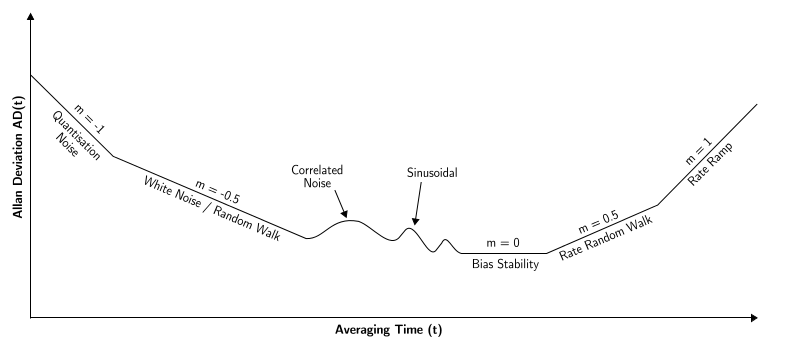
\includegraphics[width=3in]{figures/allan_regions.png}
  \DeclareGraphicsExtensions.
  \caption{The typical regions of a $\log(\textproc{Adev}(\tau))$ vs $\tau$ plot, and their relation to signal noise characteristics. Reprinted from \cite{UCAM-CL-TR-696}.}
  \label{allan_regions}
\end{figure}

\begin{figure}[!t]
  \centering
  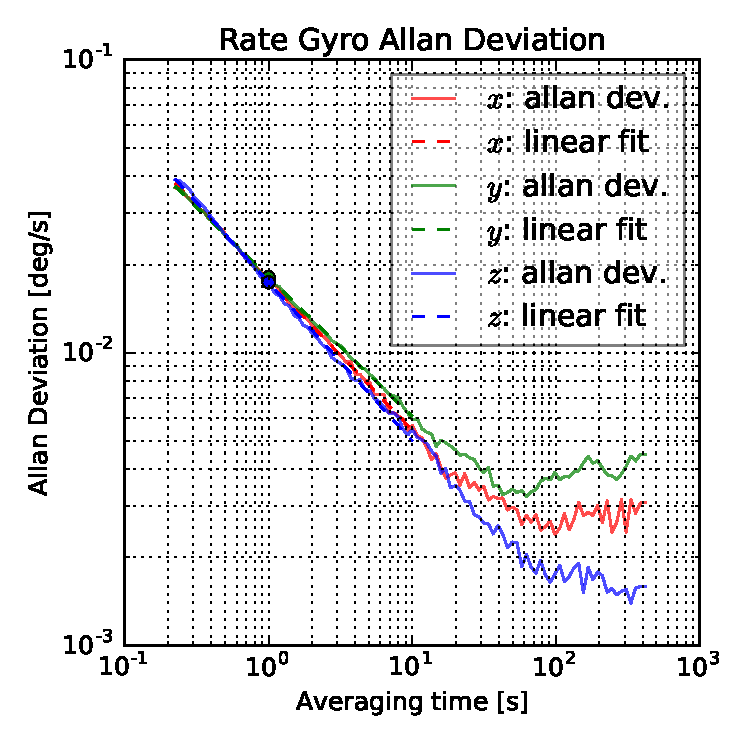
\includegraphics[width=2.5in]{figures/gyro_data_allan.pdf}
  \DeclareGraphicsExtensions.
  \caption{Allan deviation analysis of MPU-9150 rate gyroscope data.}
  \label{gyro_data_allan}
\end{figure}

\begin{figure}[!t]
  \centering
  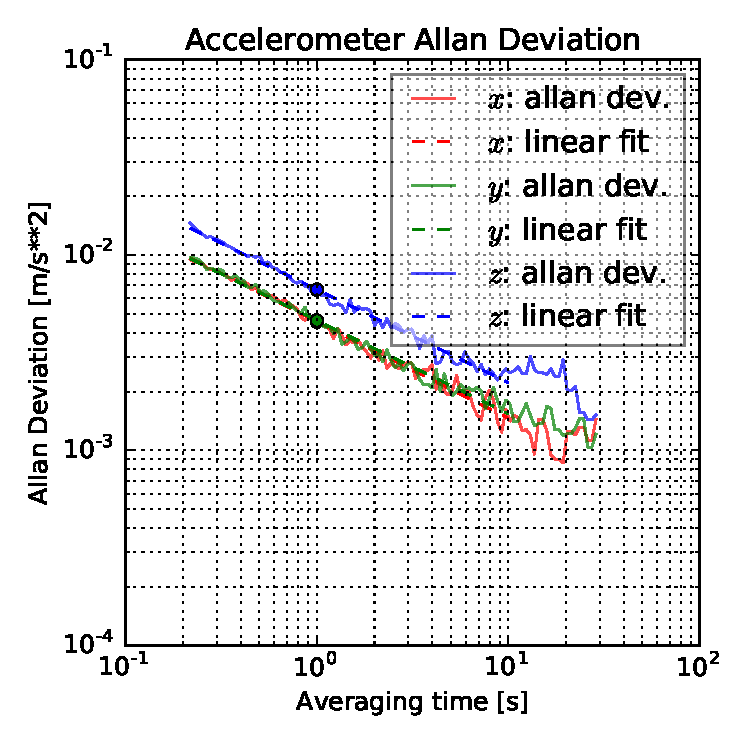
\includegraphics[width=2.5in]{figures/accel_data_allan.pdf}
  \DeclareGraphicsExtensions.
  \caption{Allan deviation analysis of MPU-9150 accelerometer data.}
  \label{accel_data_allan}
\end{figure}

\begin{figure}[!t]
  \centering
  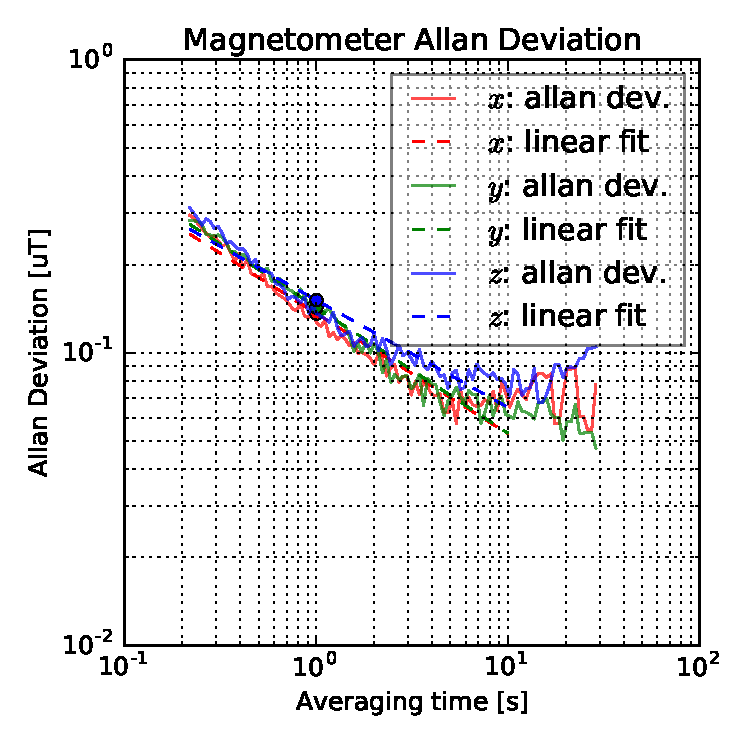
\includegraphics[width=2.5in]{figures/mag_data_allan.pdf}
  \DeclareGraphicsExtensions.
  \caption{Allan deviation analysis of MPU-9150 magnetometer data.}
  \label{mag_data_allan}
\end{figure}

The values of the sensor's noise parameters can be read from the Allan Deviation plots. The continuous-time measurement noise Fourier spectral density $\sigma_{*,c,*}$ is the value at which the linear $-0.5$ slope portion of the plot passes through $\tau = \SI{1}{\second}$ \cite{UCAM-CL-TR-696}. I perform a linear best fit on the Allan Deviation for $\tau \in [\SI{0.1}{\second}, \SI{10}{\second}]$, and find the value of the best-fit line at $\tau = \SI{1}{\second}$. For comparison, I also compute the discrete-time measurement noise $\sigma_{*,d,*}$ by taking the standard deviation of the signal. The results of both calculations are presented in table \ref{table:measurement_noise}. For all sensors, the continuous- and discrete-time noise estimates are in agreement, i.e. equation \ref{eqn:cont_to_desc_noise} is approximately correct. The accelerometer noise parameters are close to the manufacturer's specified values, while the gyro is $2$ to $4$ times nosier that the specification. The manufacturer does not specify noise parameters for the magnetometer, but my values are about $9$ times the values reported for a similar MEMS Hall effect sensor in \cite{1643403}\\

For sensor with bias walk, the Allan Deviation plot will have a flat $0$ slope region. The signal's bias instability $\sigma_{*,bi,*}$ is the minimum value of \textproc{Adev}, and the correlation time $1/\alpha$ is the value of $\tau$ at which the minimum occurs \cite{UCAM-CL-TR-696}. The continuous-time bias walk noise $\vec{\eta_u}(t)$ has standard deviation \cite{1642588}:
\begin{equation}
    \Var[\eta_{*,u,c,*}] = \sigma_{*,u,c,*}^2 = 2 \alpha \sigma_{*,bi,*}^2
\end{equation}
This is converted to discrete time by \cite{1642588}:
\begin{equation}
    \Var[\eta_{*,u,d,*}] = \sigma_{*,u,d,*}^2 = (\Delta t) (\sigma_{*,u,c,*}^2)
\end{equation}
The results of the bias walk analysis are presented in table \ref{table:bias_walk}. The accelerometer and gyro Allan Deviation plots have a flat region, indicating that a bias walk process exists for these sensors. The magnetometer Allan Deviation plot does not have a flat region, and continues at a slope of $\approx -0.5$ for all observed $\tau$. This indicates that the magnetometer does not have a bias walk process, only a white noise process. This confirms my assumption that the magnetometer bias is independent of time. The accelerometer bias is very small ($\sigma_{accel,u,c,*} \approx 10^{-4}$) compared to the quantity to be measured ($|\vec{g}_{Earth}| \approx 10$), justifying my decision to neglect bias in the accelerometer measurement model.

\begin{table*}[!t]
  % increase table row spacing, adjust to taste
  \renewcommand{\arraystretch}{1.3}
  %if using array.sty, it might be a good idea to tweak the value of
  % \extrarowheight as needed to properly center the text within the cells
  \caption{Sensor Measurement Noise Parameters. Specified parameters from \cite{mpu9150} unless otherwise noted.}
  \label{table:measurement_noise}
  \centering
  % Some packages, such as MDW tools, offer better commands for making tables
  % than the plain LaTeX2e tabular which is used here.
  \begin{tabular}{|l||c|c|c|c|}
    \hline
    Sensor & FFT noise (meas) & FFT noise (spec) & RMS noise (meas) & RMS noise (spec)\\
    \hline
    MPU-9150 Gyro $x$ axis & \SI{0.0179}{\degree\per\sqrt\second} & \SI{0.005}{\degree\per\sqrt\second} & \SI{0.125}{\degree\per\second} at \SI{46}{\hertz} & \SI{0.06}{\degree\per\second} at \SI{92}{\hertz} \\
    MPU-9150 Gyro $y$ axis & \SI{0.0162}{\degree\per\sqrt\second} & \SI{0.005}{\degree\per\sqrt\second} & \SI{0.106}{\degree\per\second} at \SI{46}{\hertz} & \SI{0.06}{\degree\per\second} at \SI{92}{\hertz} \\
    MPU-9150 Gyro $z$ axis & \SI{0.0180}{\degree\per\sqrt\second} & \SI{0.005}{\degree\per\sqrt\second} & \SI{0.141}{\degree\per\second} at \SI{46}{\hertz} & \SI{0.06}{\degree\per\second} at \SI{92}{\hertz} \\
    \hline
    MPU-9150 Accel $x$ axis & \SI{4.56e-3}{\meter\per\second\squared\sqrt\second} & \SI{3.9e-3}{\meter\per\second\squared\sqrt\second} & \SI{0.0315}{\meter\per\second\squared} at \SI{46}{\hertz} & \SI{0.039}{\meter\per\second\squared} at \SI{92}{\hertz} \\
    MPU-9150 Accel $y$ axis & \SI{4.63e-3}{\meter\per\second\squared\sqrt\second} & \SI{3.9e-3}{\meter\per\second\squared\sqrt\second} & \SI{0.0315}{\meter\per\second\squared} at \SI{46}{\hertz} & \SI{0.039}{\meter\per\second\squared} at \SI{92}{\hertz} \\
    MPU-9150 Accel $z$ axis & \SI{6.66e-3}{\meter\per\second\squared\sqrt\second} & \SI{3.9e-3}{\meter\per\second\squared\sqrt\second} & \SI{0.0453}{\meter\per\second\squared} at \SI{46}{\hertz} & \SI{0.039}{\meter\per\second\squared} at \SI{92}{\hertz} \\
    \hline
    MPU-9150 Mag $x$ axis & \SI{0.136}{\micro\tesla\sqrt\second} & Unspec'd & \SI{0.913}{\micro\tesla} at \SI{46}{\hertz} & \SI{0.1}{\micro\tesla} at \SI{100}{\hertz} \cite{1643403}\\
    MPU-9150 Mag $y$ axis & \SI{0.143}{\micro\tesla\sqrt\second} & Unspec'd & \SI{0.923}{\micro\tesla} at \SI{46}{\hertz} & \SI{0.1}{\micro\tesla} at \SI{100}{\hertz} \cite{1643403}\\
    MPU-9150 Mag $x$ axis & \SI{0.151}{\micro\tesla\sqrt\second} & Unspec'd & \SI{0.983}{\micro\tesla} at \SI{46}{\hertz} & \SI{0.1}{\micro\tesla} at \SI{100}{\hertz} \cite{1643403}\\
    \hline
  \end{tabular}
\end{table*}

\begin{table}[!t]
    % increase table row spacing, adjust to taste
    \renewcommand{\arraystretch}{1.3}
    \caption{Sensor bias walk parameters}
    \label{table:bias_walk}
    \centering
    \begin{tabular}{|l|c|c|}
        \hline
        Sensor & Bias Instability & Correlation Time \\
        \hline
        MPU-9150 Gyro $x$ axis & \SI{2.40e-3}{\degree\per\second} & \SI{98.3}{\second} \\
        MPU-9150 Gyro $y$ axis & \SI{3.23e-3}{\degree\per\second} & \SI{62.3}{\second} \\
        MPU-9150 Gyro $z$ axis & \SI{1.40e-3}{\degree\per\second} & \SI{332.0}{\second} \\
        \hline
        MPU-9150 Accel $x$ axis & \SI{7.74e-4}{\meter\per\second\squared} & \SI{57.7}{\second} \\
        MPU-9150 Accel $y$ axis & \SI{2.95e-4}{\meter\per\second\squared} & \SI{167.4}{\second} \\
        MPU-9150 Accel $z$ axis & \SI{9.91e-4}{\meter\per\second\squared} & \SI{78.2}{\second} \\
        \hline
        MPU-9150 Mag & - & $> \SI{400}{\second}$ \\
        \hline
    \end{tabular}
\end{table}



\section{Estimator Design}
Because my system has nonlinear measurements and approximately Gaussian measurement noise, I use an Unscented Kalman Filter (UKF) as my estimator.

\subsection{Quaternion State in the UKF}
The use of quaternions to represent attitude state requires some modification to the standard UKF algorithm. First, the UKF assumes
that the state space is a vector space, i.e. that all combinations of settings of the state variables are valid states. While the quaternions $\mathbb{H}$ are a 4-D vector space, only unit quaternions represent valid rotations in $\mathrm{SO(3)}$. Therefore, the attitude state space is the 3-D surface of the unit sphere in $\mathbb{H}$, i.e. it is a manifold, not a vector space.\\

This invalidates the UKF's representation of uncertainty. The distribution of states should only include unit quaternions, so level-sets of likelihood should be 3-D patches on the surface of the unit sphere (figure \ref{fig:quat_uncert_3d}. This requires a 3-D representation of the attitude covariance. However, in the UKF the dimension of the covariance is equal to the dimension of the state. Therefore, the level-sets of likelihood would be 4-D ellipsoids, and the distribution of states would include many non-unit quaternions (figure \ref{fig:quat_uncert_4d}).\\

To avoid this, the unit quaternions must be mapped to a 3-D vector space. Fortunately, the unit quaternions form a Lie group ($\mathrm{SO(3)}$), so their logarithms form a Lie algebra ($\mathrm{so(3)}$), which is a vector space (this duality is referred to as the exponential map). The logarithm of a quaternion is defined as follows: for a rotation of $\theta$ radians about a unit axis $\hat{n}$:
\begin{align}
    q &= [\cos(\frac{\theta}{2}), \hat{n} \sin(\frac{\theta}{2})] \\
    \log(q) &= [\log(|q|), \theta \hat{n}]\\
        &= [0, \theta \hat{n}]
\end{align}
The logarithm of a unit quaternion has real part 0, and complex parts equal to the axis-angle representation of the rotation. Because the real part is always zero, it can be dropped to represent the log-unit-quaternions as 3-vectors in $\mathrm{so(3)} = \mathbb{R}^3$.\\

\begin{figure}[!t]
  \centering
  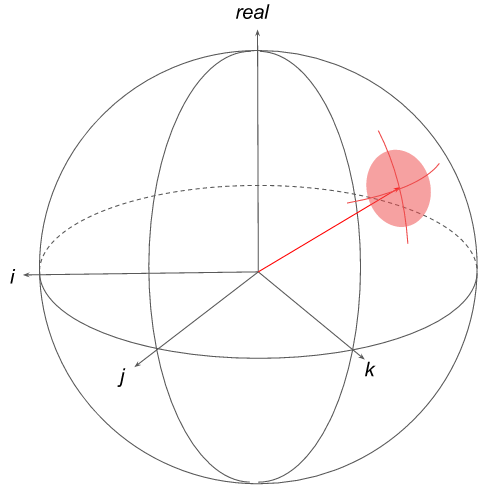
\includegraphics[width=2.5in]{figures/quat_uncert_3d.png}
  \DeclareGraphicsExtensions.
  \caption{An illustration of the 4-D unit sphere in $\mathbb{H}$, a unit quaternion (red), and its 3-D 1-$\sigma$ uncertainty region (pink). The region lies on the unit sphere.}
  \label{fig:quat_uncert_3d}
\end{figure}

\begin{figure}[!t]
  \centering
  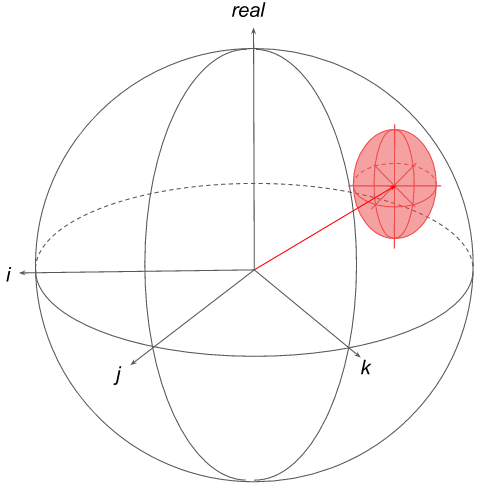
\includegraphics[width=2.5in]{figures/quat_uncert_4d.png}
  \DeclareGraphicsExtensions.
  \caption{A unit quaternion (red), and its 4-D 1-$\sigma$ uncertainty region. The region contains points which are not on the unit sphere.}
  \label{fig:quat_uncert_4d}
\end{figure}

Another issue is that the UKF must average state vectors. However, the unit quaternions are a redundant representation of $\mathrm{SO(3)}$, and a quaternion and its negative represent the same rotation. Before averaging quaternions, we must check their vector dot product, and negate one of the quaternions if it is negative.\\

\subsection{Modified quaternion UKF algorithm}
The modified quaternion UKF \cite{1257247} represents attitude uncertainty with a 3-D covariance, and uses the exponential map to convert 3-D attitude disturbance vectors to disturbance quaternions $d\mathcal{Q}^{(i)}$. Its propagation function is presented in algorithm \ref{alg:propdyn}. If there are $n$ non-attitude states, then the covariance $Q$ has dimension $(n+3) \times (n+3)$, the state estimate $\vec{x}^{est}$ has dimension $n+4$, and the sigma points $\vec{\mathcal{X}}^{(i)}$ have dimension $n+3$. States $0, 1, 2, 3$ are the attitude quaternion, other states are vector components or scalars. The diagonal entries $Q[0,0], Q[1,1], Q[2,2]$ represent the attitude estimate variance about the body-frame $x,y,z$ axes, with units of \si{\radian\squared}. $W$ is the process noise covariance, and $R$ is the measurement noise covariance.\\

\begin{algorithm}
  \caption{Quaternion UKF Dynamics Propagation.}
  \label{alg:propdyn}
  \begin{algorithmic}
    \Function{PropagateDynamics}{$\vec{x}_{k-1|k-1}^{est}, Q_{k-1|k-1}, W$}
      \State $q_{k-1|k-1}^{est} \gets \vec{x}_{k-1|k-1}^{est}[0:4]$
      \State Compute the sigma points $\vec{\mathcal{X}}^{(i)}_{k-1|k-1}$ from the covariance $Q_{k-1|k-1} + W$
      \State $d\mathcal{Q}^{(i)}_{k-1|k-1} \gets \textproc{QuatExp}(\vec{\mathcal{X}}^{(i)}_{k-1|k-1}[0:3]) \quad \forall i$
      \State $\mathcal{Q}^{(i)}_{k-1|k-1} \gets q_{k-1|k-1}^{est} \cdot d\mathcal{Q}^{(i)}_{k-1|k-1} \quad \forall i$
      \State Propagate each state vector $[\mathcal{Q}^{(i)}_{k-1|k-1}, \vec{\mathcal{X}}^{(i)}_{k-1|k-1}[3:]]$ through the state transition function to step $k|k-1$.

      \State $q_{k|k-1}^{est} \gets \textproc{QuatAvg}(\mathcal{Q}^{(i)}_{k|k-1} \quad \forall i)$
      \State $\vec{x}_{k|k-1}^{est}[0:4] \gets q_{k|k-1}^{est}$
      \State $\vec{x}_{k|k-1}^{est}[4:] \gets \textproc{Mean}(\vec{\mathcal{X}}^{(i)}_{k|k-1}[3:] \quad \forall i)$

      \State $d\mathcal{Q}^{(i)}_{k|k-1} \gets (q_{k|k-1}^{est})^{-1} \cdot \mathcal{Q}^{(i)}_{k|k-1}$
      \State $\vec{\mathcal{X}}^{(i)}_{k|k-1}[0:3] \gets \textproc{QuatLog}(d\mathcal{Q}^{(i)}_{k|k-1})$
      \State Compute $Q_{k|k-1}$ from $\vec{\mathcal{X}}^{(i)}_{k|k-1}$

      \Return $\vec{x}_{k|k-1}^{est}, Q_{k|k-1}$
      \EndFunction
  \end{algorithmic}
\end{algorithm}

\begin{algorithm}
  \caption{Quaternion UKF Measurement Update.}
  \label{alg:updatemeas}
  \begin{algorithmic}
    \Function{UpdateMeasurement}{$\vec{x}_{k|k-1}^{est}, Q_{k|k-1}, \vec{y}_{k}, R$}
      \State $q_{k|k-1}^{est} \gets \vec{x}_{k|k-1}^{est}[0:4]$
      \State Compute the sigma points $\vec{\mathcal{X}}^{(i)}_{k|k-1}$ from the covariance $Q_{k|k-1}$
      \State $d\mathcal{Q}^{(i)}_{k|k-1} \gets \textproc{QuatExp}(\vec{\mathcal{X}}^{(i)}_{k|k-1}[0:3]) \quad \forall i$
      \State $\mathcal{Q}^{(i)}_{k|k-1} \gets q_{k|k-1}^{est} \cdot d\mathcal{Q}^{(i)}_{k|k-1} \quad \forall i$
      \State Map each state vector $[\mathcal{Q}^{(i)}_{k|k-1}, \vec{\mathcal{X}}^{(i)}_{k|k-1}[3:]]$ through the measurement function to get the measurement sigma points $\vec{\mathcal{Y}}^{(i)}_{k}$.
      \State $\vec{y}^{est}_{k} = \textproc{Mean}(\vec{\mathcal{Y}}^{(i)}_{k} \quad \forall i)$
      \State Compute $Q_{yy}$ from $\vec{\mathcal{Y}}^{(i)}_{k}$ and $R$.
      \State Compute $Q_{xy}$ from $\vec{\mathcal{X}}^{(i)}_{k|k-1}$ and $\vec{\mathcal{Y}}^{(i)}_{k}$.
      \State $K \gets Q_{xy} Q_{yy}^{-1}$
      \State $d\vec{\mathcal{X}} \gets K (\vec{y}_{k} - \vec{y}^{est}_{k})^T$
      \State $dq = \textproc{QuatExp}(d\vec{\mathcal{X}}[0:3])$
      \State $q_{k|k}^{est} \gets q_{k|k-1}^{est} \cdot dq$
      \State $\vec{x}^{est}_{k|k}[0:4] \gets q_{k|k}^{est}$
      \State $\vec{x}^{est}_{k|k}[4:] \gets \vec{x}^{est}_{k|k-1}[4:] + d\vec{\mathcal{X}}[3:]$
      \State $Q_{k|k} \gets Q_{k|k-1} - K Q_{yy} K^T$

      \Return $\vec{x}_{k|k}^{est}, Q_{k|k}$
    \EndFunction
  \end{algorithmic}
\end{algorithm}

\subsection{Sensor Bias Estimation}
I augment the system state $[q_{NED2sensor}, \vec{\omega}^{sensor}]$ with the gyroscope and magnetometer bias parameters $[\vec{b}, \vec{h}^{sensor}_{bias}]$ and run the UKF on the augmented state. This allows the biases to be estimated on-the-fly without the need for pre-calibration. It also accounts for the time-varying nature of the gyroscope bias. However, this approach requires the system to be in motion. The system's absolute rotation about the gravity vector is only observable though magnetometer measurements. If the system does not move, only one ($\pm$ noise) magnetometer measurement is observed. From this single measurement, it is impossible to determine both the magnetometer bias parameters and the rotation about $\vec{g}$. Once measurements from several different orientations have been collected, the estimator has sufficient information to determine both the rotation about $\vec{g}$ and the magnetometer bias.

\section{Results}
\subsection{Simulation Results}

\subsection{Experimental Results}



\section{Conclusion}
mag model insufficient % better model: http://www.acsu.buffalo.edu/~johnc/mag_cal05.pdf.





% conference papers do not normally have an appendix


% trigger a \newpage just before the given reference
% number - used to balance the columns on the last page
% adjust value as needed - may need to be readjusted if
% the document is modified later
\newpage
\IEEEtriggeratref{8}
% The "triggered" command can be changed if desired:
%\IEEEtriggercmd{\enlargethispage{-5in}}

% references section

% can use a bibliography generated by BibTeX as a .bbl file
% BibTeX documentation can be easily obtained at:
% http://mirror.ctan.org/biblio/bibtex/contrib/doc/
% The IEEEtran BibTeX style support page is at:
% http://www.michaelshell.org/tex/ieeetran/bibtex/
\bibliographystyle{IEEEtran}
% argument is your BibTeX string definitions and bibliography database(s)
\bibliography{IEEEabrv,16322_report}


% that's all folks
\end{document}


